\documentclass[tikz,border=10pt]{standalone}
\usetikzlibrary{matrix,arrows.meta}
\tikzset{
  centered/.style = { align=center, anchor=center },
     empty/.style = { font=\sffamily\Large, centered, text width=2cm },
       box/.style = { font=\sffamily, fill=green, centered },
       input/.style = { font=\sffamily, fill=black!20, centered },
    result/.style = { font=\sffamily\scriptsize, fill=black!20, centered},
     arrow/.style = { very thick, color=red, ->, >=Triangle},
}
\newcommand*{\nothing}{Do nothing}
\begin{document}
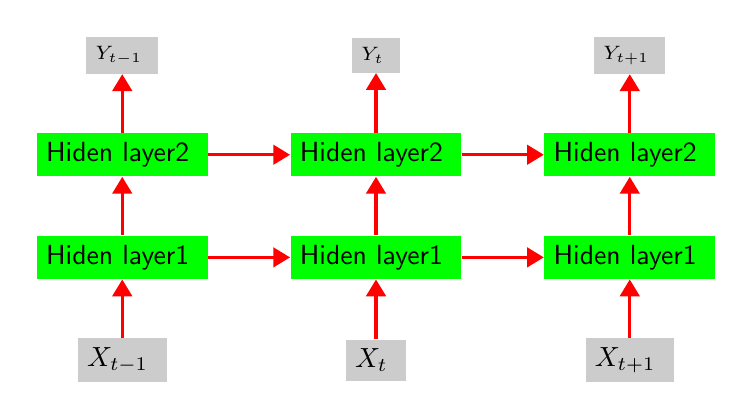
\begin{tikzpicture}
  \matrix (m)
    [
      matrix of nodes,
      column sep      = 3em,
      row sep         = 5ex,
      row 1/.style = { nodes = { result }  },
      row 2/.style = { nodes = { box }    },
      row 3/.style = { nodes = { box } },
      row 4/.style = { nodes = { input } },
    ]
    {
      $Y_{t-1}$  & $Y_t$ & $Y_{t+1}$ \\
      Hiden layer2  & Hiden layer2 & Hiden layer2 \\
      Hiden layer1  & Hiden layer1 & Hiden layer1 \\
      $X_{t-1}$  & $X_t$ & $X_{t+1}$ \\
    };
  \foreach \i/\j in {1/2,2/3,3/4} {
    \draw [arrow] (m-\j-3) -- (m-\i-3);
    \draw [arrow] (m-\j-2) -- (m-\i-2);
    \draw [arrow] (m-\j-1) -- (m-\i-1);
  }
  \foreach \i/\j in {1/2,2/3} {
    \draw [arrow] (m-2-\i) -- (m-2-\j);
    \draw [arrow] (m-3-\i) -- (m-3-\j);
  }
\end{tikzpicture}
\end{document}